\chapter{System implementation}

In this chapter we will discuss the actual implementation of the original idea
behind Linkero: a brand monitoring case management application. We will start
from the architecture in order to show a general snapshot of the system, before
talking in details about every single component, the technology that was
chosen and reasons behind. We will follow with use cases and
system requirements, to conclude with class diagram, database structure and some
code samples.

\section{System architecture}
The system achitecture figure \ref{sysarch} here below provides an overview of
all different applications that work together to provide the main system
functionalities.

\begin{figure}[h!]
\centering
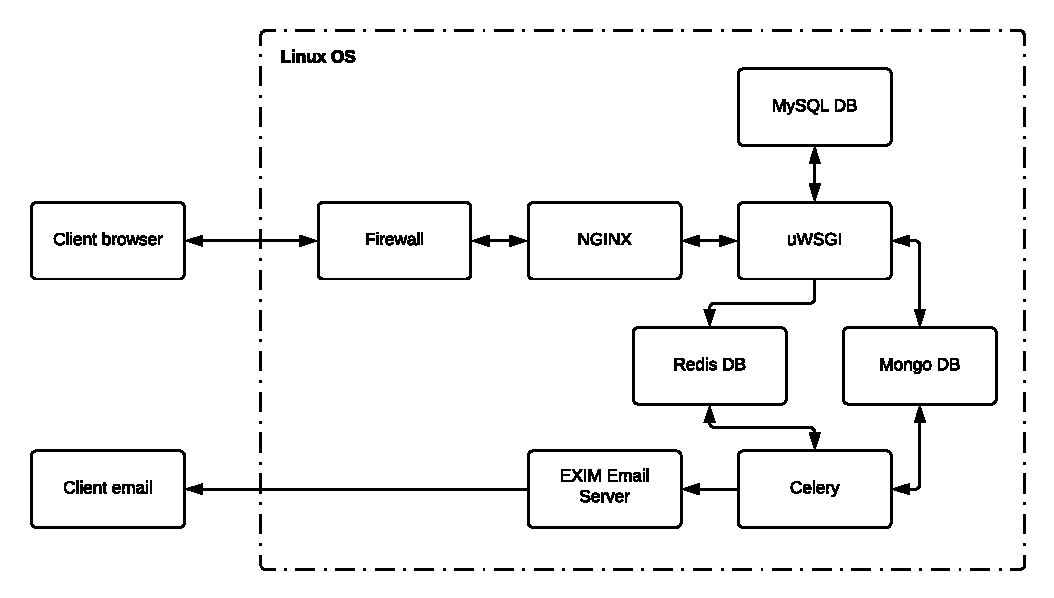
\includegraphics[scale=0.8]{imgs/SystemArchitecture.pdf}
\caption{Linkero system architecture}
\label{fig:sysarch}
\end{figure}

As shown in the figure, client browser and client email are considered part of
the system: the former becuase some functionalities are passed to the client to
run locally in the form of JQuery functions, and the latter because it represent
the final destination of data files generated bythe system.

Linux is the operating system running on a Virtual Private Server, that manages
all other applications. The first point of entry is the Firewall, which monitors
all requests knocking ports 22, 80 and 443.

NGINX is the web server, reverse proxy server \cite{WikiNginx}, which receives
HTTP requests and assigns them to the correct internal web server.

uWSGI is the web server that runs Python scripts, in the words of its
developers: ``uWSGI itself is a vast project with many components, aiming to
provide a full software stack for building hosting services'' \cite{RtduWsgi}.

Python scripts from within uWSGI can make calls to three databases. MySQL keeps
information about users registration details, passwords, and access logs. Mongo
DB instead is used to store all the data generated by users with their queries.
Finally Redis DB simply stores information about tasks that have been scheduled
and that will run independently from uWSGI's scripts.

Celery is another server running Python scripts scheduled by the main web
server. It does so by regularly checking in Redis if any new task has been
logged, and if that's the case it will execute each task sequentially.

Finally the email server is only called for outgoing emails, to deliver a copy
of all the data collected in a .csv file attached to the email.

\section{Technologies}

\subsection{Server operating system}

\subsection{Web application framework}

\subsection{Databases}

\subsubsection{Maria DB}

\subsubsection{Mongo DB}

\subsubsection{Redis DB}

\subsection{Web engine}
NGINX was chosen to serve the pages of this application.

\subsection{Firewall}

\section{Development methodology}

\section{Use cases}

\begin{figure}[h!]
\centering
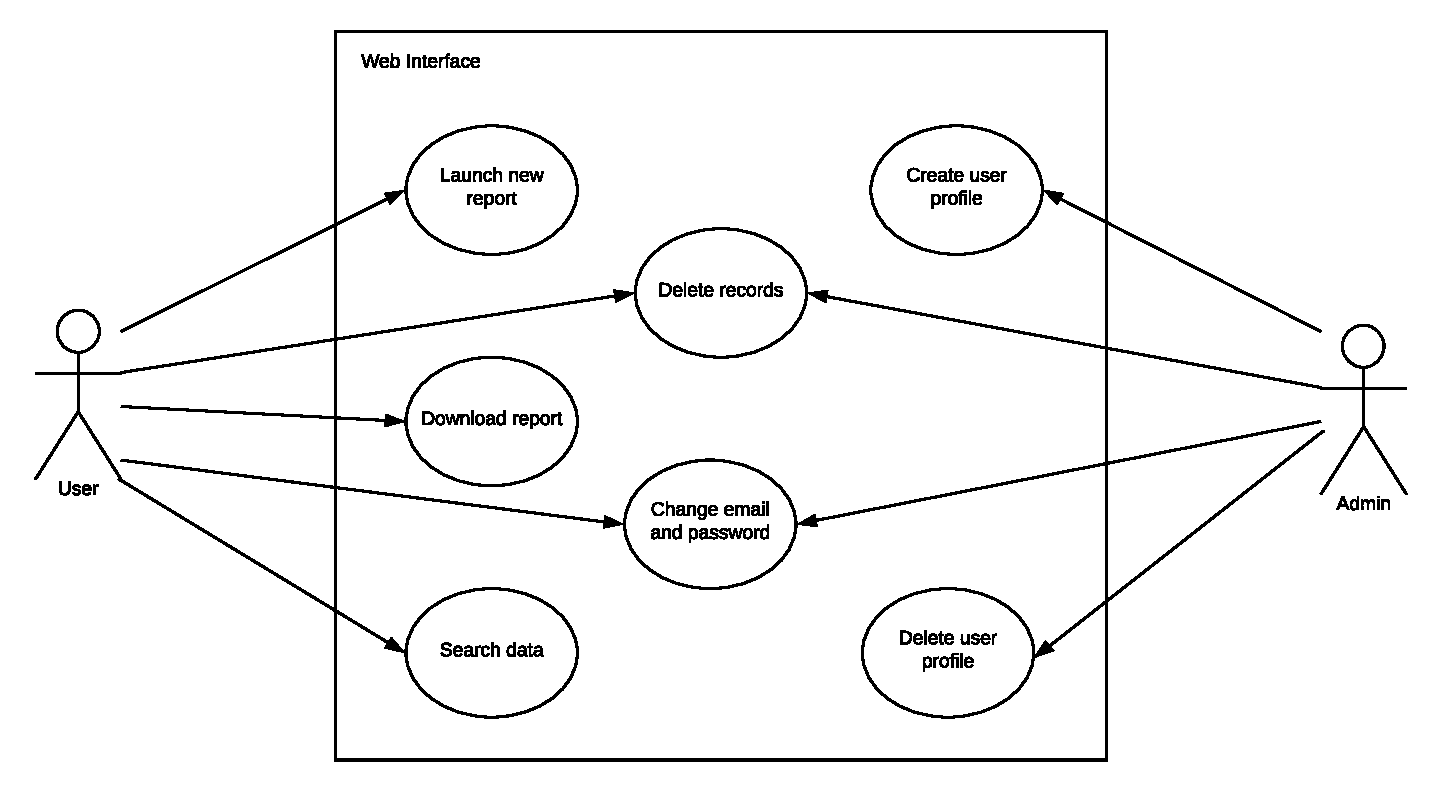
\includegraphics[scale=0.4]{imgs/UseCasesDiag.pdf}
\caption{Use cases diagram}
\label{fig:sysarch}
\end{figure}

\section{Requirements}

\subsection{Functional requirements}

\subsection{Non-functional requirements}

\subsection{User requirements}

\subsection{Requirements analysis}

\section{Sequence diagrams}

\begin{figure}[h!]
\centering
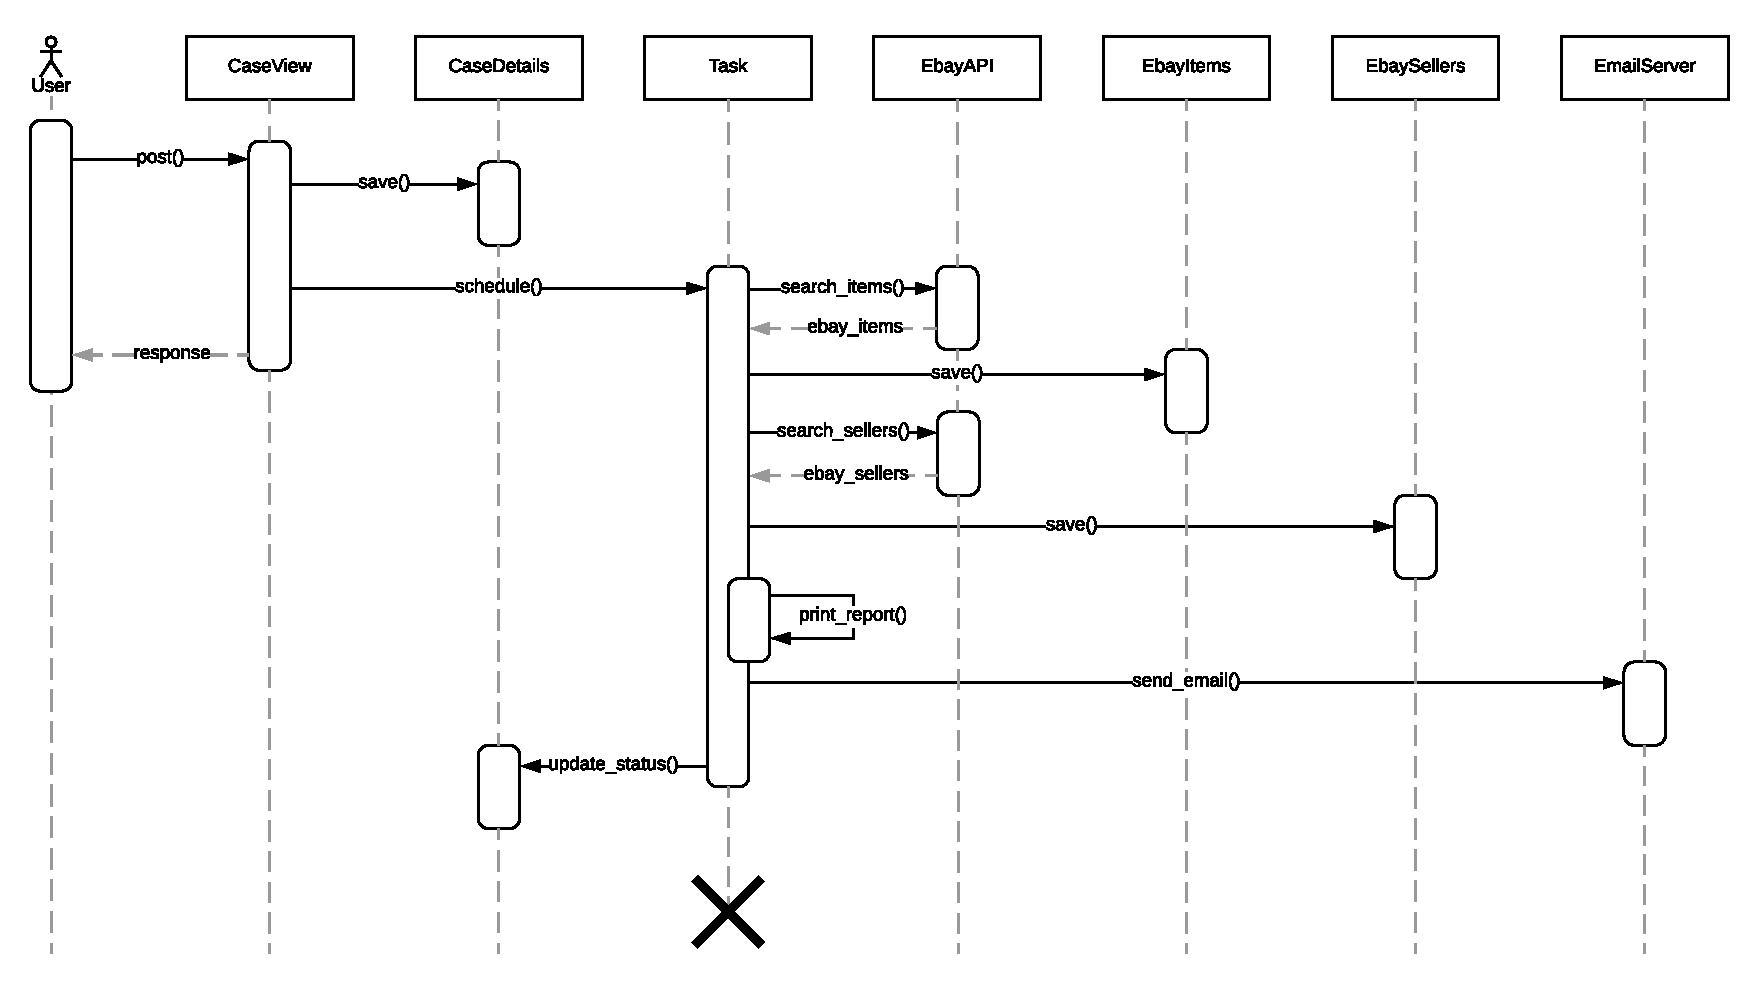
\includegraphics[angle=90, scale=0.7]{imgs/SequenceDiagram.pdf}
\caption{Launch report sequence diagram}
\label{fig:sysarch}
\end{figure}

\section{Code samples}
